
\documentclass{acm_proc_article-sp}
%\documentclass{sig-alternate}
\usepackage{hyperref}
\usepackage{cite}

\begin{document}

%\conferenceinfo{AISec}{'15 Denver, Colorado, USA}
\conferenceinfo{XXXX}{'15 XXXX, XXXXXXXXXXXX, USA}

\title{IFuzzer: An evolutionary fuzzer using genetic programming}
\numberofauthors{2} 
\author{
\alignauthor
Spandan Veggalam\\
       \affaddr{IIIT Hyderabad,India}\\
       \email{
       veggalam.s@reseach.iiit.ac.in}
\and
% 2nd. author
\alignauthor
Sanjay Rawat\\
       \affaddr{IIIT Hyderabad,India}\\
       \email{sanjay.rawat@iiit.ac.in}
}
\maketitle

\begin{abstract}
A vulnerability is a weakness in a system, technology or design. Fuzzing is an automated black box testing used for finding security vulnerabilities in the software by providing random data as input. Input programs must be digestible i.e. semantically valid to pass the Interpreter elementary checks. On the other hand, the fuzzed input must also be indigestible so as to trigger the uncommon behavior of the Interpreter. In our IFuzzer approach we use evolutionary computing techniques in the area of interpreter fuzzing. IFuzzer uses grammatical evolution techniques and guides the fuzzer in generating indigestible input code fragments that may trigger exceptional behavior of interpreter such as crashes, memory leaks and failing assertions. IFuzzer uses language grammar to generate digestible inputs and is an effective tool: applied on JavaScript interpreter which found 22 vulnerabilities in the time span of one month.
\end{abstract}

\category{}{Security and Privacy}{Systems Security}[Vulnerability detection]
\terms{SECURITY, VERIFICATION}
\keywords{Security, Fuzzing, JavaScript, Grammatical Evolution, Evolutionary Computing, 
Genetic Algorithms, Artificial Intelligence, Interpreters}

\section{Introduction}
Software security is essential dimension for a software. Web browsers are one of the application software serves as an interface for different networks and many systems. These browsers are becoming more and more sophisticated, thereby render different services for which they include several inter-connected components. Interpreters are of one such component for languages like JavaScript, PHP, Flash, PDF, XSLT and many more. Because of their widespread usage, they became primary applications for security attack, data and privacy breaches. The interpreters included can be exploited for launching browser based security attacks \cite{Sekar09}. JavaScript is one such widely used interpreter responsible for several vulnerabilities. We look at such attacks in the following perspective:
\begin{enumerate}
\item The way of handling information which includes extracting, parsing, storing, manipulating and communicating may also raise some vulnerabilities.
\\e.g., Cross Site Scripting
\item Flaws in browser software components like script engines, plug-ins, etc., can be used to exploit vulnerabilities. 
\item Browser components may also result in low-level vulnerabilities which can be exploited.
\\e.g., memory corruptions, assertion failures, uncommon behaviors etc.
\end{enumerate}
\indent The Web has proved to interlink different information systems and has become main medium for sharing information. In the recent past, there have been numerous studies, techniques, and tools proposed mainly to address the security issues related to information processing.	However, in the context of web related vulnerabilities particularly software's like browsers and their components, not much has been investigated in the direction of the above mentioned point 2. As a result, recently, there have been many bugs uncovered in browser-run software's: e.g., DOM Components, PDF interpreters, JavaScript Engines.\\
\indent Fuzz testing is a useful approach for finding vulnerabilities in software. One of its variants, evolutionary fuzzing, turned out to be a useful smart fuzzing method. These methods make use of evolutionary computing approaches to automatically generate inputs that exhibit vulnerabilities.\\
\indent Interpreter fuzzers must generate syntactically valid input, otherwise inputs will not pass the elementary interpreter checks. Therefore input must be generated making use of knowledge about target language. Assuming JavaScript interpreter to be target, fuzzed input must follow the syntax specifications of JavaScript language. Otherwise JavaScript interpreter discards the inputs during its first step i.e., parsing. Therefore JavaScript language grammar is used to generate syntactically valid code fragments. With built-in language grammar valid data can be modeled. Both language dependent and independent fuzzers can be built with some additional knowledge of a specific language. \textit{jsfunfuzz} \cite{Jesse07} is popular fuzzer for Mozilla's JavaScript engine. This is an example for language dependent fuzzer. Another fuzzer \textit{Langfuzz} \cite{Holler11} is an example of language independent fuzzer generates syntactically valid code fragments. With the motivation from this language independent fuzzer - can we map LangFuzz approach to genetic programming paradigm?\\
\indent In this paper we will introduce a new framework called \textit{IFuzzer}, that generates code fragments using Grammatical Evolution methods, a particular form of Genetic Programming \cite{Neill_10}, thereby allows black box fuzzing of the Interpreters. IFuzzer takes language's context free grammar as input for tests generation, for instance given JavaScript grammar it generates JavaScript programs; also uses grammar to learn code fragments from the input code base. Given a test suite, IFuzzer performs standard genetic algorithm  operations; crossover and mutations on the input code fragments and uses learnt code fragments for replacements - Grammatical Evolution brings transparency on making decision, inspired by biological evolution. It follows Darwin's theory of evolution and selects programs with high fitness. Here, objective function favors the program which are uncommon enough and likely to trigger interpreter exceptional behaviors and are selected for fuzzing. Grammatical Evolution approach is appropriate at generating code, and likely to produce diverse code fragments.\\

\begin{figure}
\centering
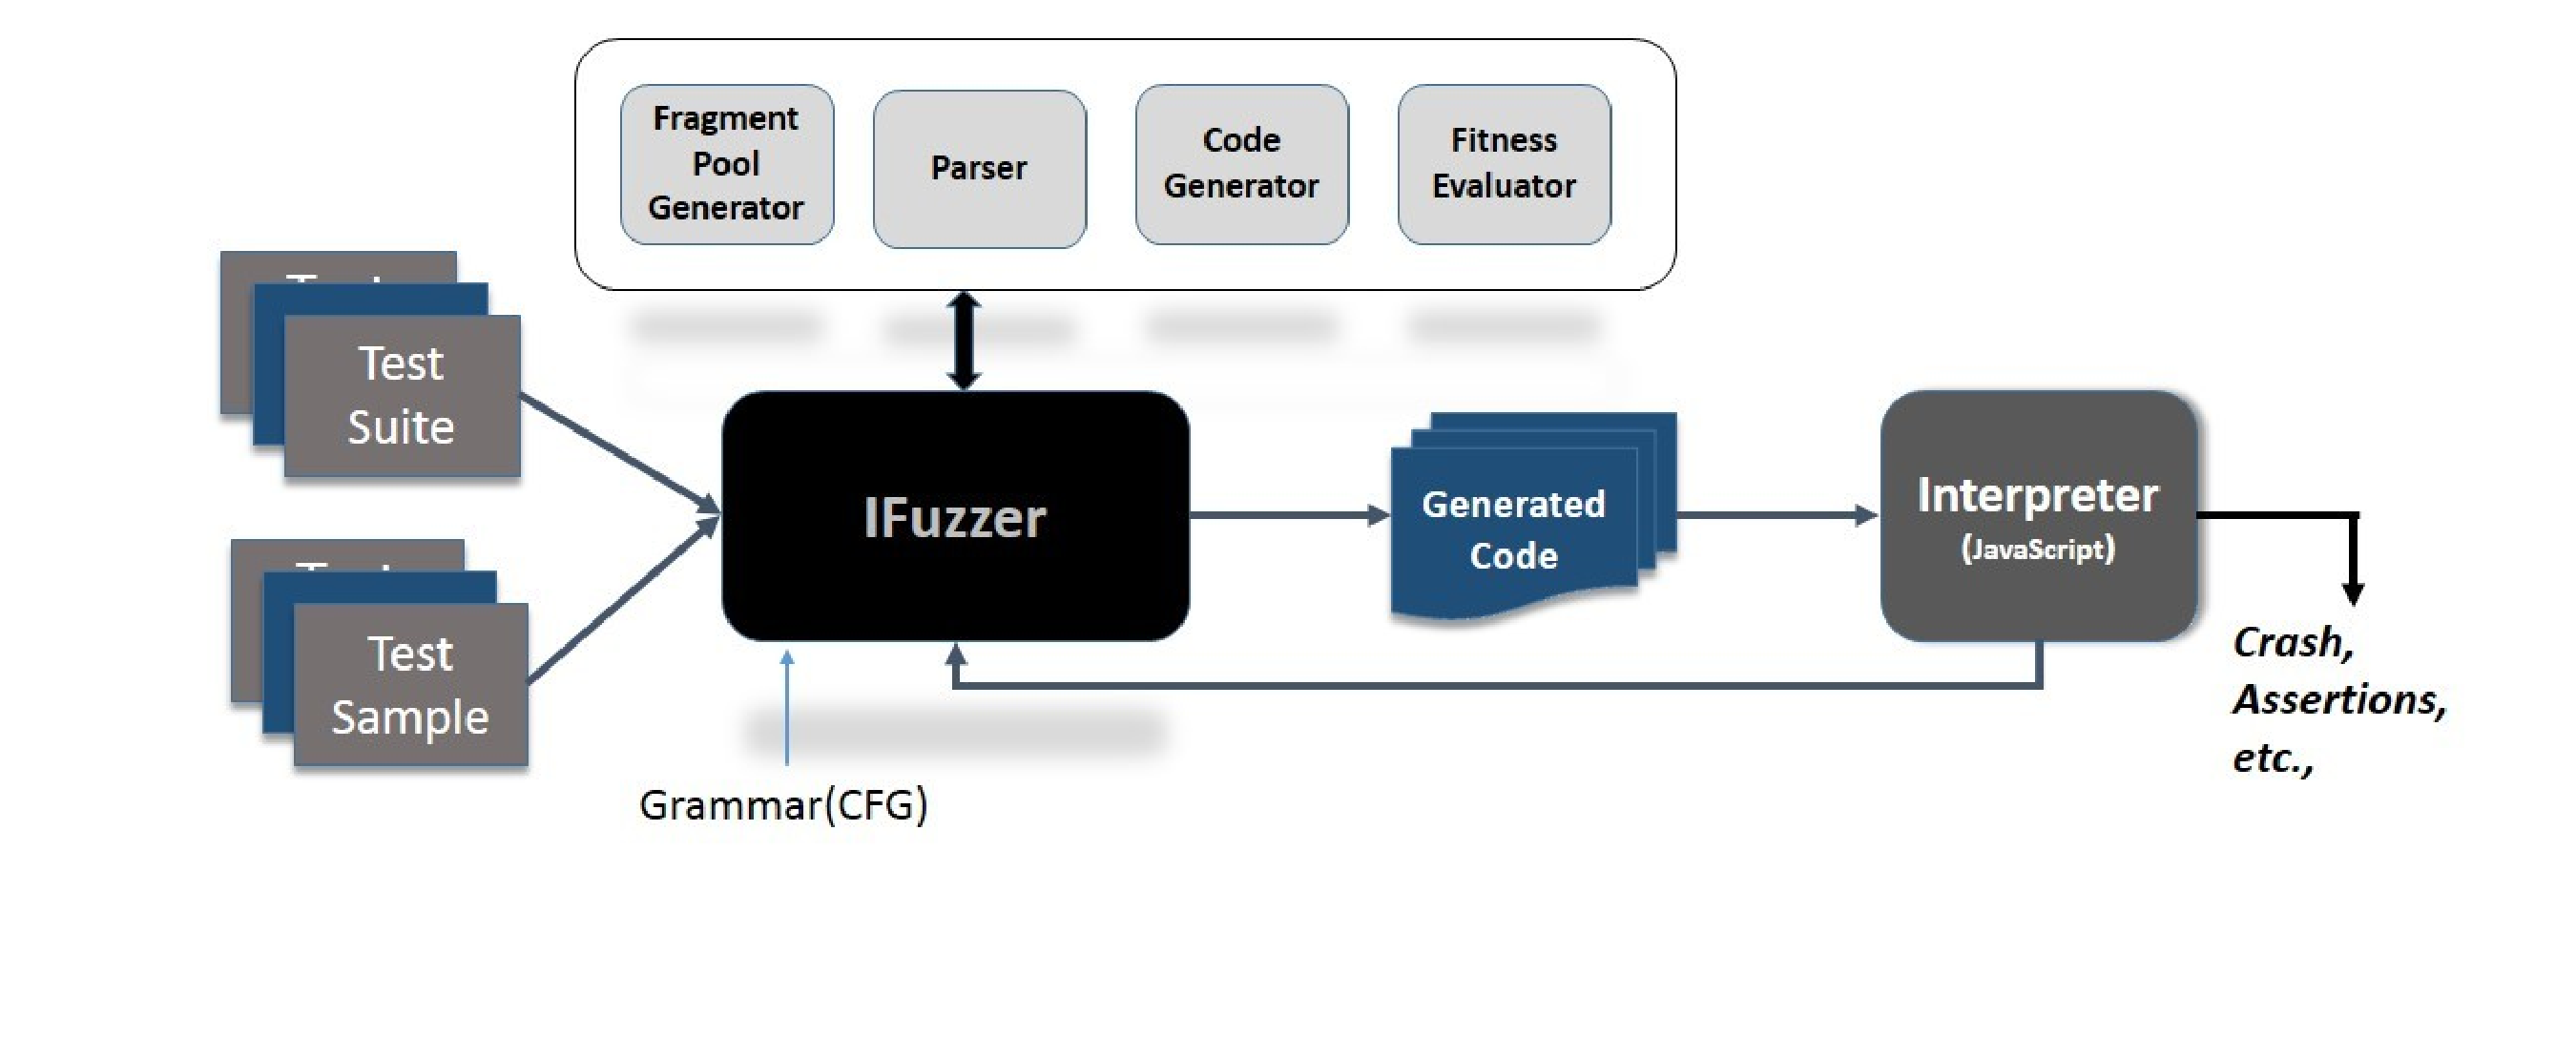
\epsfig{file=process.eps, height= 2in, width=3.8in}
\caption {Overview of IFuzzer Approach}
\medskip
Describes the overview of IFuzzer which takes test suite, language grammar and sample code as input. Language grammar is used to parse the program. Language grammar is used to parse the program. CodeFragment extractor extracts code fragments for non-terminals. GECodeGenerator generates code fragments.
\label{fig1}
\end{figure}

\indent  Figure \ref{fig1} describes the overview of IFuzzer which takes test suite, language grammar and sample code as input. Parser uses language grammar to parse the program and generates XML object as abstract syntax representation. Fragment pool of code fragments is formed by parsing each input file from sample codes. Input test suite itself can also be used as sample codes. IFuzzer generates new code fragments by performing genetic operations on the test suite. \\
\indent Remaining paper explains the code generation process and fuzzing process. ~\autoref{bk} presents the motivation for choosing Grammatical Evolution for code generation. In ~\autoref{GEIF} we describe the methods involved in code generation process. Implementation of IFuzzer is discussed in ~\autoref{impl}.~\autoref{eval} discusses the experimentation setup and evaluation step of IFuzzer and ~\autoref{conclusion} closes with conclusion.

\section{Background} \label{bk}
\subsection{Related Work}
Fuzz testing started as naive approach of directing random data towards program interface, but it is proved to be effective at uncovering bugs. Started as project to test Unix system utilities with random input, at University of Wisconsin Madison in 1989 by Professor Barton Miller \cite{Miller89}. Miller and his students were among the first to develop fuzzer for real time interfaces. Since then fuzzer is widely adopted by different communities. It was transformed from small recess technique to one that is widely adopted techniques. \\
\indent Researchers started fuzzers as brute forcing tools for discovering flaws, after which they would analyze for possibility of security exploitation. After many years it was realized that such simple approaches have many limitations in discovering complex flaws \\
\indent Studies on genetic programming and its application in code generation, and code generations for interpreter and compiler testing  are relevant to this work. In 2001 Kaksonen \cite{Kaksonen} in his approach \textit{mini-simulation}, used simplified description of protocols and syntax to automatically generate inputs that nearly matches with the protocol usage. This approach is generally called as grammar based approach, provides the fuzzer with sufficient information to understand protocol specifications. Kaksonen's \textit{mini-simulation} is used to ensure the protocol checksums are always valid and also systematically checks which rules are broken. \\
\indent Fuzzing the compilers and interpreters requires random fuzzing strategies for discovering bugs. In 2011, Yang et al \cite{Yang} presented their work on CSmith, a random c program generator tool uses grammar for producing programs with different features. \\
\indent Zero-day vulnerability forced the researchers to pay more attention on software security. Similar vulnerabilities of web browsers and its components are increasing rapidly. This made security testing on web browsers and interpreters promising. JsFunFuzz \cite{Jesse07} is a language dependent generative tool written by ruddersman in 2007, targets JavaScript interpreters in web browsers and has lead to discovery of more than 1800 bugs in Spidermonkey, firefox's JavaScript engine. It is considered as most relevant work in this field. In 2012, Langfuzz written by Holler at el \cite{Holler11} is an language independent tool used language grammar and code mutation approaches for test generation.\\
\indent In 2011, Zalewski presented ref\_fuzz \cite{Zelaski08} and cross\-fuzz \cite{Zelaski11} tools aiming DOM component in browsers. He revealed interesting problem with the modern web browsers. Zelaski also published fuzzers for different browser components and found several bugs.\\
\indent There are few proprietary fuzzers targeting different software components. Google's ClusterFuzz \cite{Arya12} one of such fuzzer tests different functionalities in Chrome. It is tuned to generate almost 5 million tests in a day and have found several unique vulnerabilities in chrome components.\\
\indent However these approaches may deviate the process of code generation from generating required test data, thereby degenerates into random search and provides low code coverage.\\ 
\indent Feedback fuzzers adjusts and generates dynamic inputs based on information from the target system, \textit{Evolutionary Fuzzer} is one example of this kind. Evolutionary fuzzing uses evolutionary algorithms to create required search space of data and operates based on a objective function that takes the control of test input generation. One of the first published approaches to evolutionary fuzzing \cite{demott2007} is from Michigan State University by DeMott et al. 2007. This a Grey-box technique that measures code block coverage and generates new inputs generation-ally with better code coverage to find bugs. Inspired with LangFuzz's language independent approach in security fuzzing, we adapted the idea of evolutionary algorithms in IFuzzer for test generations.

\subsection{Terminology}
In the following sections we make use of following terminology.

\begin{enumerate}
\item{\textbf{Interpreter.}} In this paper the term \textit{"Interpreter"} is software system that executes input program. This translates code from one form to other form during execution. 
\item{\textbf{Genotype.}} In this paper the term \textit{"Genotype"} refers to an  object that carries information of the individuals, taking part in evolution process. 
\item{\textbf{Phenotype.}} In this paper the term \textit{"Phenotype"} refers to the structure of the program that is  directly executed and on which fitness is calculated based on the behavior of this individual.
\item{\textbf{Grammar.}} The grammar defines the context free grammar of the target language. Grammar is defined in backus normal form or extended backus normal form.
\item{\textbf{Genome.}} In grammatical evolution genome is the linear representation of an individual. All the genetic operators are applied on this linear representation and plays vital role in evolution process.
\item{\textbf{Codon.}} \textit{Co-don} is building block of Genome. Each codon is of equal size. 
\item{\textbf{Search Space.}} Search space is the set of all feasible solutions. Each point is the represents a solution defined by fitness values or some other values related to an individual. 
\item{\textbf{Bug/Defect.}} In this paper the term \textit{bug} or \textit{defect} refers to an abnormal behavior of the target software system (e.g. Crash due to memory overflows, assertion failures, etc.) 
\end{enumerate}

\section{IFuzzer Approach} \label{GEIF}
In this section we discuss how to use Grammatical Evolution(GE) Techniques \cite{Ryan98},\cite{Ryan00},\cite{Ryan01},\cite{PoliLM2008} for program generation. In general testing inputs are generated using Generative approaches or Mutation approaches or both. \textit{IFuzzer} makes use of both mutation and generative approaches. IFuzzer follows Grammatical evolution approach in code generation. Grammatical Evolution is a Genetic Programming(GP) paradigm and analogous to biological evolutionary process. Grammatical Evolution applies genetic operators crossover, mutation and replacements on the individuals in program generation process. In this process of evolution all Genotypes are mapped to Phenotypes \cite{Fagan10}. 

\subsection{Representation}
Genetic programming and Grammatical Evolution differs in the way the inputs are represented. Genetic programming is confined to use tree structures for program representations. Various variants of GP are proposed based on program representations. GE doesn't pose any constraints on structure generally follows linear representations like strings, binary string etc., IFuzzer follows binary string representation of the genotypes \cite{Hugosson10} which is referred as genome. Each genome of genotype contains codons of 8bit length, which are used in selecting production rules form the grammar. For eg., JavaScript variable statement \textit{var s;} is represented in binary representation as follows.
\begin{center}
\textbf{var s};\\
\textbf{1100110101010111100100111101001001010110}\\
{\small (Example of Genotype in binary representation)}
\end{center}

\indent All the genetic operations are applied to this linear structure, unlike they are applied to tree like structures in traditional GP approach which follows tree like representations.
\subsection{Fragment Pool}
From the set of files code from input code base fragment pool is formed by extracting code fragments for each non terminal in the language grammar. In this phase, we process each input file by the language parser. Using the parser, code fragments are extracted from the input files. Each code fragment is represented by a non-terminal. With sufficient number of input files, code fragments can be generated to all non-terminals in the language grammar. These code fragments are used in mutation and code generation phase, same logic is followed in crossover for identifying code fragments for selected common non-Terminal between the participating individuals. \\
\indent In mutation code fragments in the input is replaced with corresponding non-terminal code fragment selected from the fragment pool. In crossover code fragments of same type from two different programs are exchanged with each other. All these operations may be semantically invalid  or not useful in the context of input programs involved in different phases. For this we perform semantic improvement and new code fragments are generated in context of participating individual semantics

\subsection{Initial Population}
A set of initial population of individuals are generated by randomly selecting certain number of programs equal to population size from the input test samples. This forms first generation of evolution. After each generation individuals forms the parental set of individuals (genotypes) which undergo genetic operations, and their by evolves into off-springs enforcing to maximum size of population.
Genetic algoritms uses many parameters, of them crossover, mutation rate and population size are basic paramters. Their values are set based on hueristics. Small changes to the values may adversely affect the evolution process and deviates it from the objective. There are few other parameters that control the process. 

\subsection{Genetic Operators}
In this section we will look into how the genetic operators are implemented in IFuzzer. ~\autoref{fig3} illustrates the crossover and mutation operations over binary strings. After each operation, the off-spring evolved is evaluated for the fitness by the objective function defined. Fitness evaluation is further discussed in ~\autoref{fitness}.

\begin{figure*}
\centering
\epsfig{file=crossover.eps, height= 2.1in, width=4.5in}
\caption {(a). Single point Crossover (b). Multiple point Crossover }
\label{fig2}
\end{figure*}

\begin{figure*}
\centering
\epsfig{file=mutation.eps, height= 1.3in, width=4.5in}
\caption {(a). Multiple point Mutation (b). Single point Mutation }
\medskip
Mutation and Crossover illustration on binary string at boundary of similarity
\label{fig3}
\end{figure*}

\subsubsection{Crossover}
In Grammatical Evolution Crossover \cite{Ryan03} is analogous to biological operation, performed on string based linear structure(Genome) and is considered to be an exploratory operator. Types of crossover operations are differentiated based on number of crossover points. In our approach we perform  homologous two point crossover on two individuals by swapping code fragments that belongs to same non-terminal. Following steps are followed:

\begin{enumerate}
\item Randomly two individuals are picked from the population. 70\% of time we use only the top half of the sorted list to pick parents and in remaining 30\% of time we consider entire population 
\item Parse the two individuals that undergo crossover by the language parser. \item Identify list of common non-terminals based on set of code fragments that can be formed from the individuals.
\item A non-terminal is randomly selected from the list of common non-terminals. 
\item Code fragment of common non-terminal is randomly selected from both the individuals is exchanged with each other. More than one code fragment in an individual may be an example of selected common non-terminal.
\item Typically 1..3 non-terminals are randomly selected (for crossover) in this process. 
\end{enumerate}

\subsubsection{Mutation}
Mutation considered as divergence operator \cite{Byrne10}, brings diversity among the population and improves the search space. It brings structural changes to individuals and has benificial impact on search space traversals. Here, Mutation is performed by replacing code fragment with different code fragments of similar type. For this we pick some of code fragments randomly from the fragment pool and replace them with the code fragments of same type. Replacement is performing by selecting code fragment from the pool or before replacing them directly, we perform some improvements to the structure as discussed in ~\autoref{cgen}. Selected code fragment is replaced with one formed by expanding the non-terminal using the corresponding production rules from language grammar. After expansion all the non-terminals are converged to terminals. Typically mutation is performed by randomly selecting 1..3 non-terminals.

\subsubsection{Shrink Mutation and Hoist Mutation}
Apart from mutation we perform Shrink mutation in which we replace a randomly chosen code fragment with a terminal or we remove the code fragment completely. As with Hoist Mutation code fragment is selected from the complete program and is considered as complete program for next generation. In both shrink and hoist mutation, it is motivated by the desire to reduce program size. 

\subsubsection{Replacement}
During the process of off-spring generation, it is important to retain the features of best chromosomes (parents) participating in evolution. Therefore Fitness elitism method is followed to retain the best chromosomes among the parents, and these chromosomes are included as the off-springs. For this set of chromosomes in fitness sorted order are forwarded to next generations untouched. Remaining off-spring population is formed with the ones generated from crossover and mutation. This prevents the loosing the best ones in the process.

\subsection{Bloat Control}  \label{bloat}
Bloating \cite{PoliLM2008} is a phenomenon that adversely effects in evolutionary computing. Bloating is distinguished into two types: functional and structural bloating. \\
\indent In practical after some point of time the average size of programs start growing rapidly due to uncontrolled growth \cite{Soule96}. This results in inefficient code and growth doesn't relate to improvements in fitness. On the other hand, large programs require more computation to process. This is because code modification in a region may result in inviable code that perform no function or it may result in large code which do not change fitness at all. This is structural bloating.\\
\indent In functional bloating \cite{LangdonP98} range of fitness values become narrow and thereby reduces the search space. Though it is common to have different individuals with same fitness but because of bloating after some time everything looks linear and it becomes hard to distinguish individuals.\\
\indent Bloat control \cite{Luke06} can be applied at different stages and applying at the level of the fitness evaluation is very common technique. We use parsimony pressure \cite{SouleF98}, ad-hoc method for combating the bloat. With this method the selection probability of the individual by penalizing the larger ones i.e. fitness is re-calculated with some penalty depending on their size. Bloat control is also applied at breeding level uses shrink mutation and fair size crossover \cite{PoliLM2008} techniques. We use following bloat control techniques.

\subsubsection*{\textbf{Fitness e-calculation using Parsimony Co-efficient}} \label{p_co-ef}
Fitness value of the individual is re-calculated with some penalty using following equation:
\[f_{new}(x) = f(x) - penalty  \]
Penalty is the product of parsimony co-efficient and length of individual. Here length of abstract structure is considered as length of individual.
\[penalty = c*(l(x))\]
where \textit{l(x)} is length of abstract syntax structure i.e. XML Object, \textit{c} is the parsimony co-efficient or parsimony penalty computed dynamically. Following equation is used to calculate parsimony co-efficient \textit{c(t)} at each generation \textit{t}:
\[ c(t) = \frac{Covariance(f,l)}{Variance(l)}\]
\[ c(t) = \frac{\sum_{i=0}^{n}(f_{i}-\bar{f})(l_{i}-\bar{l})}{n-1} X  \frac{n-1}{\sum_{i=0}^{n}(l_{i}-\bar{l})^2}\]
where $\bar{l}$ and $\bar{f}$ are mean fitness and length of all individuals in population respectively, $f_{i}$ and $l_{i}$ are original fitness and length of individual \textit{i}.\\
\indent $Covariance(f,l)$ calculates the co-variance between individual's fitness and length, $Variance(l)$ gives the variance in the length of the individuals respectively.

\subsubsection*{\textbf{Fair Size Generation}}
Fair size generation limits the growth of the offspring's with bias value. In our approach we restrict the percentage of increase in program non-terminals to certain biased value. In other way we reject the individual. This is repeated for certain number of iterations before discarding. 
\[length_{generated\_code}/length_{original\_code} < bias_{threshold}\]
\indent where length gives information about of number of non-terminals in parse tree and bias is the threshold value for fair size generation. In this way we restrict the growth of program, if the program generated fails to meet this constraint program it is discarded as invalid and the program is re-generated

\subsection{Code Evolution} \label{cgen}
With Crossover and Mutations, we generate diverse code fragments and order of genetic operations is purely random either of mutation or crossover can take place first. \\ 
\indent Using language parser parses the input program and returns the abstract syntax tree represented by an XML structure. Tags in XML object are formed with language non-terminals and text embedded between tags is the code fragment identified from input program according to language syntax. All the non-terminals nested and ordered according to input program structure. Extracting the text in the order of XML structure re-generates input program itself. \\
\indent During mutation method, several random code fragments part of input program are selected for mutation. Removing the selected non-terminal form an incomplete program and voidness of this code fragment is filled by code fragment that can be identified by non-terminal or non-terminal is expanded to complete program. We use following expansion algorithm:

\begin{enumerate}
\item Following steps are executed in loop up to a depth \textit{d}
\begin{enumerate}
\item Set of non-Terminals in the incomplete program are identified.
\item Identify the set of productions $P_{n}$ $\subset$ P under the non-Terminal \textit{n}.
\item Modulo operation on the number of productions with decimal integer of codon, a production \textit{p} is selected. 
\[p_{rule-selected} = codon mod number-of-rules\]
\item Replace the non-terminals occurrence with \textit{p}.
\item Gene string is appended to itself in case of in sufficient codon values.
\end{enumerate}
\item After expanding to a certain depth \textit{d}, all the remaining non-terminal occurrences are to be replaced with terminals to yield complete program. For this we randomly select same type of code fragments from fragment pool.
\item[] Codons are the chunks of 8-bits from the gene of the individual.
\end{enumerate}

\indent In Crossover, several random fragments (Typically 1..3) are selected from the both the individuals by selecting common non-terminals from the corresponding XML objects. These selected fragments from one individual are exchanged with fragments of other individual. All these operations are performed on XML objects, after which new programs are generated from these modified XML objects.\\
\indent Genetic operators mutation or crossover or both performed on the population in each generation and thereby forms off-spring population i.e. next generation. Code generation process is continuous process and is terminated after a certain number of generations or based on stopping criteria. \\
\indent With primary target to trigger exceptional behavior of the Interpreters and Compilers, we start with existing test cases written for the target language by developers as a standard practice. All the  processes discussed above are applied to the test cases one after one, from the learning phase to mutation phase, thereby creating executables from the original test cases.

\subsection{Semantic Adjustment} \label{semantics}
In our Language Independent approach, we try to generate semantically valid programs by maintaining semantical context of the input programs. Introducing language semantics ties IFuzzer to a language specifications. Code fragments generated with Crossover, Mutation and Initial Population generation   methods might be semantically invalid or out of semantic context of original inputs. We perform generic class of semantic transformations as part of small semantic adjustments at syntactic level. \\
\indent Continuation of semantics is one such generic approach can be used to any programming language. Re-using literals occurred in body of input programs is an example of this approach. With this we can reducing undeclared identifier exceptions. In most of the languages all the memory locations and functions are named with identifiers and are declared somewhere in the body of the program. These identifiers must be declared before they are used, but in some languages like JavaScript they can be declared anywhere in the program and are evaluated during run time. Re-using the identifiers from the body of the original input within the new fragments reduce the chances to have undeclared identifiers. This can be done at the syntactic level. For this IFuzzer need to know the identifiers used in the input program, from the language grammar using identifier non-terminal we identify the identifiers from the program and replace identifiers in new fragments. It is still possible that identifiers are undeclared at the time of executing (because the reused identifier may be declared downward the new fragment) but the chance of undeclared identifier is reduced. \\
\indent IFuzzer is aware of the language global objects and built in functions which can be used with out declaring them. List of these objects and functions are passed as an argument with which they are identified in the new fragments. These objects are left unmodified by IFuzzer, are usually defined in the implementation of language.

\subsubsection*{\textbf{SemiColon Insertion}}
Semantic Adjustment discussed above with small additions can be a language independent adjustment. Another adjustment we make is Automatic Semicolon Insertion is language specific approach performed based on ECMAScript-262 specifications \cite{EcmaScript}. According to grammar some JavaScript statements must be terminated with semicolons and are therefore affected by automatic semicolon insertion. 

\begin{figure*}
\centering
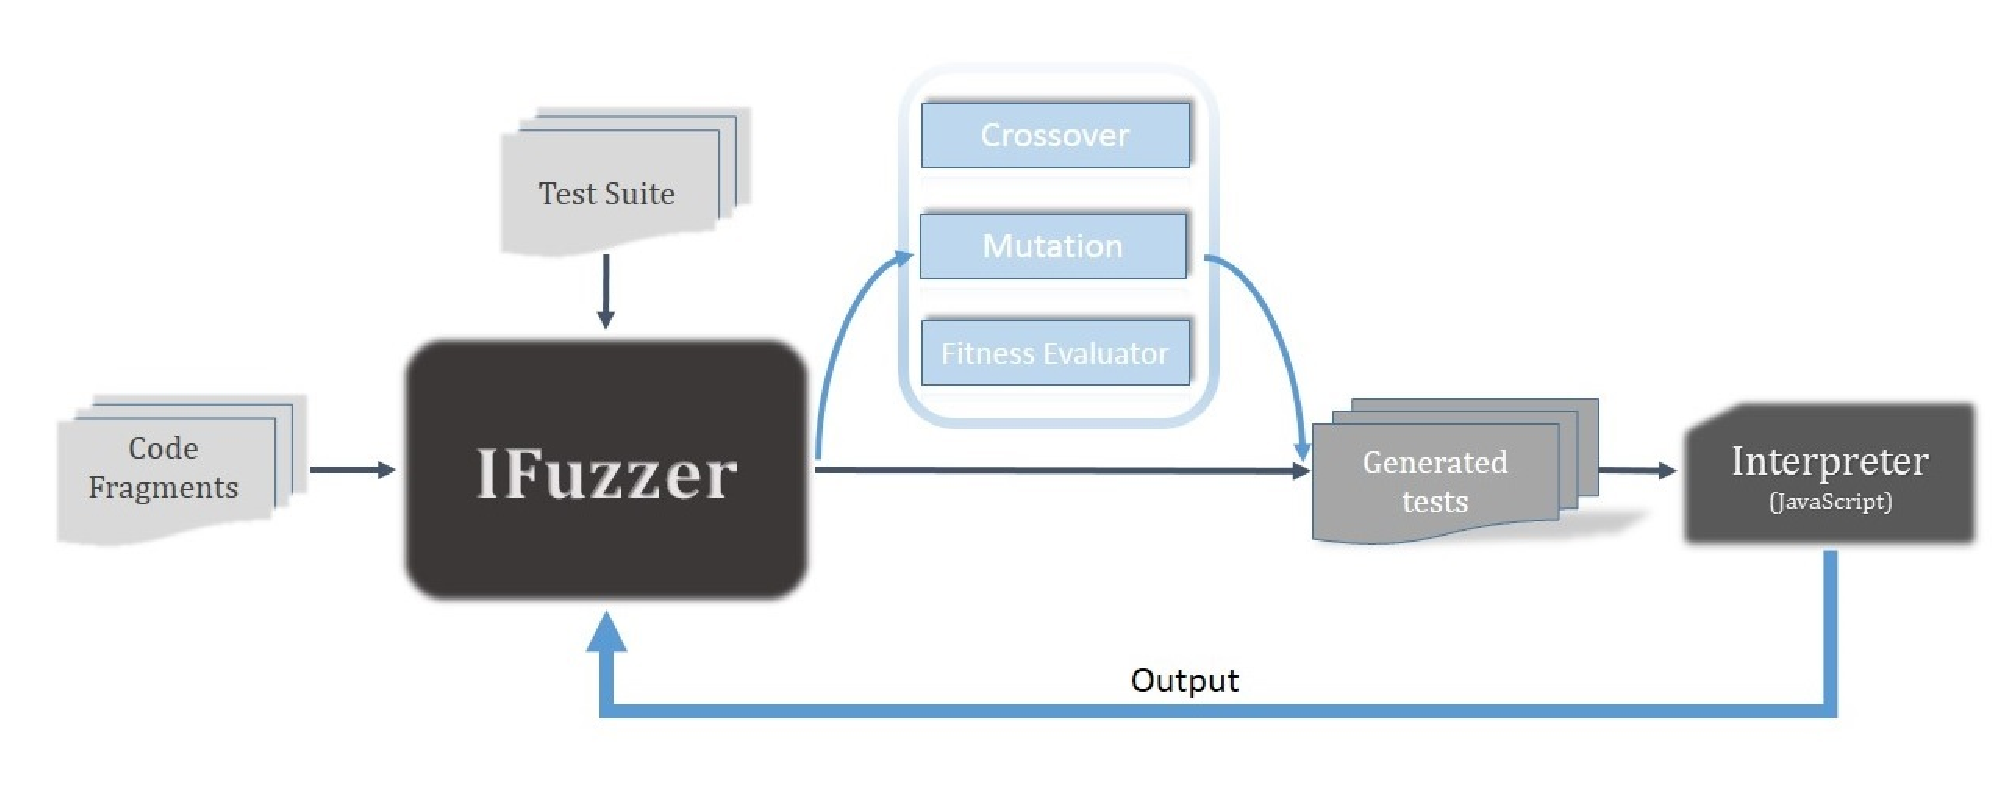
\epsfig{file=process1.eps, height= 2.55in, width=6.5in}
\caption {Overview of IFuzzer Approach}
\medskip
 describes the overview of IFuzzer which takes test suite, language grammar and sample code as input. Language grammar is used to parse the program. Parser uses language grammar to parse the program. 
\label{fig4}
\end{figure*}

\section{Implementation} \label{impl}
A fuzzer is implemented as proof-of-concept based on all the methods discussed so far and works as described in overview diagram ~\autoref{fig1} in the introduction. IFuzzer starts with Fragment Pool generation process, where it takes each input file from the test suite and extracts code fragments for different non-terminals in language grammar.
After extracting fragments from all input file, fuzzer starts it code generation and fuzzing process. 

\subsection{Parser}
In most of the discussed methods input code is parsed and corresponding XML structure is generated. For this, IFuzzer uses ANTLR parser generator framework \cite{Parr13} to generated parsers for different languages using grammar specified in BNF. Why Antlr? Because of its easy-of-use over performance and different parse generation options which automatically build trees that can be folded into any application. Parser is used to extract code fragments from input test suite or to generate abstract syntax for which in either cases parser generates XML object as abstract syntax of program. Code fragments are extracted for each non-terminal from these XML objects. XML objects are involved in fragment pool generation and code generation methods.

\subsection{Code Generation}
IFuzzer uses ANTLR parser for target language which generated using ANTLR language grammar. As discussed in ~\autoref{cgen} Crossover, Mutation and Initial Population generation methods make use of XML objects returned by the parser for performing their operations. Small simplifications are made to grammar syntax internally without making any semantic changes and also changes are made to introduced Identifier as non-terminal (In most of ANTLR grammars identifier is included as terminal fragment). This makes step-wise expansion algorithm discussed in ~\autoref{cgen} easier and newly introduced identifier non-terminal simplifies semantic adjustment and identifiers listing process. \\
Grammar simplification includes following modifications:

\begin{enumerate}
\item Rules containing sub-alternatives are written as separate rules.
\item All the rule quantifiers and optionals are removed by introducing additional rules.
\end{enumerate}
Additional rule created are added to corresponding non-terminals. After these simplifications all the rules are left with non-terminals and terminals.\\
\indent During Initial population creation itself, identifiers are extracted for particular individual and cached for further processing. In Code generation process, new fragments are fitted into existing semantic-al context as explained in ~\autoref{semantics}. For this purpose IFuzzer uses the cached identifiers for replacing the identifiers in new fragments. For suppose if an identifier "a" in new fragment is replaced with "b", all the occurrences of "a" are replaced with "b". Local Identifiers are mapped to Global and built-in identifiers but vice versa will not happen.\\
Code generation process is continued for a number of generations or until a individual with target fitness value is generated. 

\subsection{Fitness Evaluation} \label{fitness}
Evolutionary process is an objective driven process therefore fitness function that defines the objective of the process plays an vital role in code generation process. Individual's fitness is calculated at different stages. After crossover and mutation phases generated the code fragments are evaluated. Fitness value is calculated based on different factors. Various program parameters which includes structure of program, warnings raised by the interpreter, crashes, execution time outs, singularity are considered as fitness parameters. For instance nested (or complex) structure have tendency to create uncommon behaviour, so it gains more score compared to less complex structured programs. Each parameter $J_{k}$ in the fitness function is associated with a weight $w_{j}$ determined based on the observations. For each individual $I_{i}$, we define the fitness as follows:
\[score_{i} = \sum_{j=0}^{k} w_{j} * f_{ij} \]
\[F_{i} = score_{i} + singularity_{i}  \]
where $f_{ij}$ is the occurrence frequency or characteristic value of parameter, singularity of the individual is calculated at the point of mutation based on the selection and expansion of non terminals. W is the set of weights for each parameter. Selection of values in W is of predominant important for fitness function and are decided based on heuristics.\\
\indent As discussed in \autoref{bloat} fitness is re-calculated with some penalty which is product of parsimony co-efficient \textit{c} and the length of individual \textit{l}. Fitness is re-calculated at each generation using following equation:
\[f_{new}(x) = f(x) - c*(l(x))  \]
where $f_{new}(x)$ and $f(x)$ are new and old fitness values of an individual $x$.

\subsection{Executing tests}
IFuzzer executes the test inputs generated after each GA methods discussed. Valid test cases are considered for fitness evaluation. IFuzzer requires to generate more number of population generations thereby and after each iteration code generation moves towards the more desired solution. Here the objective is to identify uncommon behavior of interpreter with valid inputs. All the tests are performed in the persistent shell of the interpreter and uncommon behaviors are traced. \\
\indent In case of failure due to invalid code fragment or if program doesn't meet Fair Size bias constraint discussed in \autoref{bloat}, Mutation and Crossover operations try to re-generate programs till it generates valid programs and gives up the re-generation process after certain number of trails. \\
\indent IFuzzer contains many adjustable grammatical evolution parameters, e.g. mutation rate, crossover rates, population size, number of generations and many others. All the default values are derived from experiments. We tried to use the best combination based on observations, but these doesn't promise the certainty to deliver the best performance. It is not feasible to compare all parameter combinations because the evaluation of parameter set is time consuming. After a change in a paramter set it takes hours (or days) to evaluate, so repeating the process several times and observing the process to compare the results is not practical to do easily. In Table ~\autoref{AppendixA} we listed the important parameters and their default values.\\
\indent  Delta Debugging algorithm \cite{DeltaTool} is used to filter out the irrelevant code from the test case resulting in small test cases, thereby part of test case that is relevant to failure \cite{ZellerH02} is filtered out. This algorithm reduces the number of lines of code executed and  results in suitably small code fragment that causes failure.

\section{Experimentation} \label{eval}
In our experiment, we used Mozilla development test suite as input which consists of 3000-3200 programs. Same test suite is used for fragment pool generation and program generation. Fragment Pool generation is one time process, all the programs are read at the start of fuzzer and fragments are extracted for different non-terminals. This test suite is assumed to have triggered exceptional behavior at some point time earlier in development cycles. Grammar rules are written from ECMAScript 262 specification \cite{EcmaScript} and for latest version Javascript engines we include more rules that are part of the Mozilla's ECMAScript 6,7 (Harmony) development \cite{EcmaScript2}.

\subsection{LangFuzz vs IFuzzer}
Langfuzz written by holler at el \cite{Holler11}, is mutative fuzzer for testing interpreters. This is playing active part in Mozilla's and other companies QA activities and this product is integrated as part of mozilla development process.\\
\indent There are significant differences between Langfuzz and IFuzzer. Langfuzz is a mutation fuzzer and as it is provided with grammar specifications makes it adaptable to test any interpreter. To be language independent it compromises the semantic level adaption during code generation process but in order to generate valid programs it makes certain semantic level adjustments. This gives the flexibility to remain as language independent tool and need not bother about the new features induced in the language. Langfuzz easily incorporates these features from the updated grammar specifications. This means that

\begin{enumerate}
\item Langfuzz is solely dependent on the language grammar, with some additional semantic knowledge.
\item Changes to language features doesnt require any additional product development, other than grammar updates.
\end{enumerate}

\indent In contrast, IFuzzer is a guided fuzzer, with an objective is to trigger unexceptional behavior of the interpreters. IFuzzer remains as language independent tool and incorporates the evolution strategies in code generation process. \\
\indent Both IFuzzer and LangFuzz are generative fuzzers uses grammar to be language independent and differs in code generation process. LangFuzz uses mutative approaches where as IFuzzer uses grammatical evolution technique for code generation. This makes fair comparison difficult. 

\subsection{Environment Setup}
We choose \textit{Spidermonkey} as a target Interpreter for JavaScript. The main reason for choosing Spidermonkey is, Mozilla development process and related artifacts are publicly available. For all the tests, we used Mozilla's development repository and the test cases as first set of input. Input grammar specification is written from ECMAScipt standard specification. We decided to choose Spidermonkey 1.8.5 as comparison base. The main reason for choosing this version is to have comparison with LangFuzz. This version of Spidermonkey is in development by the time Holler presented his work on LangFuzz \cite{Holler11}. All the bugs found by LangFuzz during its initial development where listed in holler presentation with bug id's filed in Mozilla's bugzilla tool. In each instance we ran our application for 4-6 hours before making any changes to parameters which guides the fuzzer to reach goal. All the parameters of code generation are selected based on heuristics. When ever a bug is found we analyze it for cause and check whether it is identified by the LangFuzz during the period it targeted that specified version.  

\begin{figure}[h]
\centering
\rule{9cm}{0.5pt}
\epsfig{file=codesnippet.eps, height= 0.8in, width=3.9in}
\rule{9cm}{0.1pt}
\caption {Test Case generated by IFuzzer crashing the Spidermonkey JavaScript engine with an internal assertion when executing line 4.}
\label{fig6}
\end{figure}

\subsection{Result of Comparison}
During the experiment, we ran many instances in a span of one month. IFuzzer found  a total of 22 unique different bugs during this period. In contrast, to the 51 bugs listed in LangFuzz presentation which are found during it initial runs of 4 months. There are three overlapped bugs found by both LangFuzz and IFuzzer this addresses the research question "How many overlapped bugs are found by both fuzzers?". 

\begin{figure}[h]
\centering
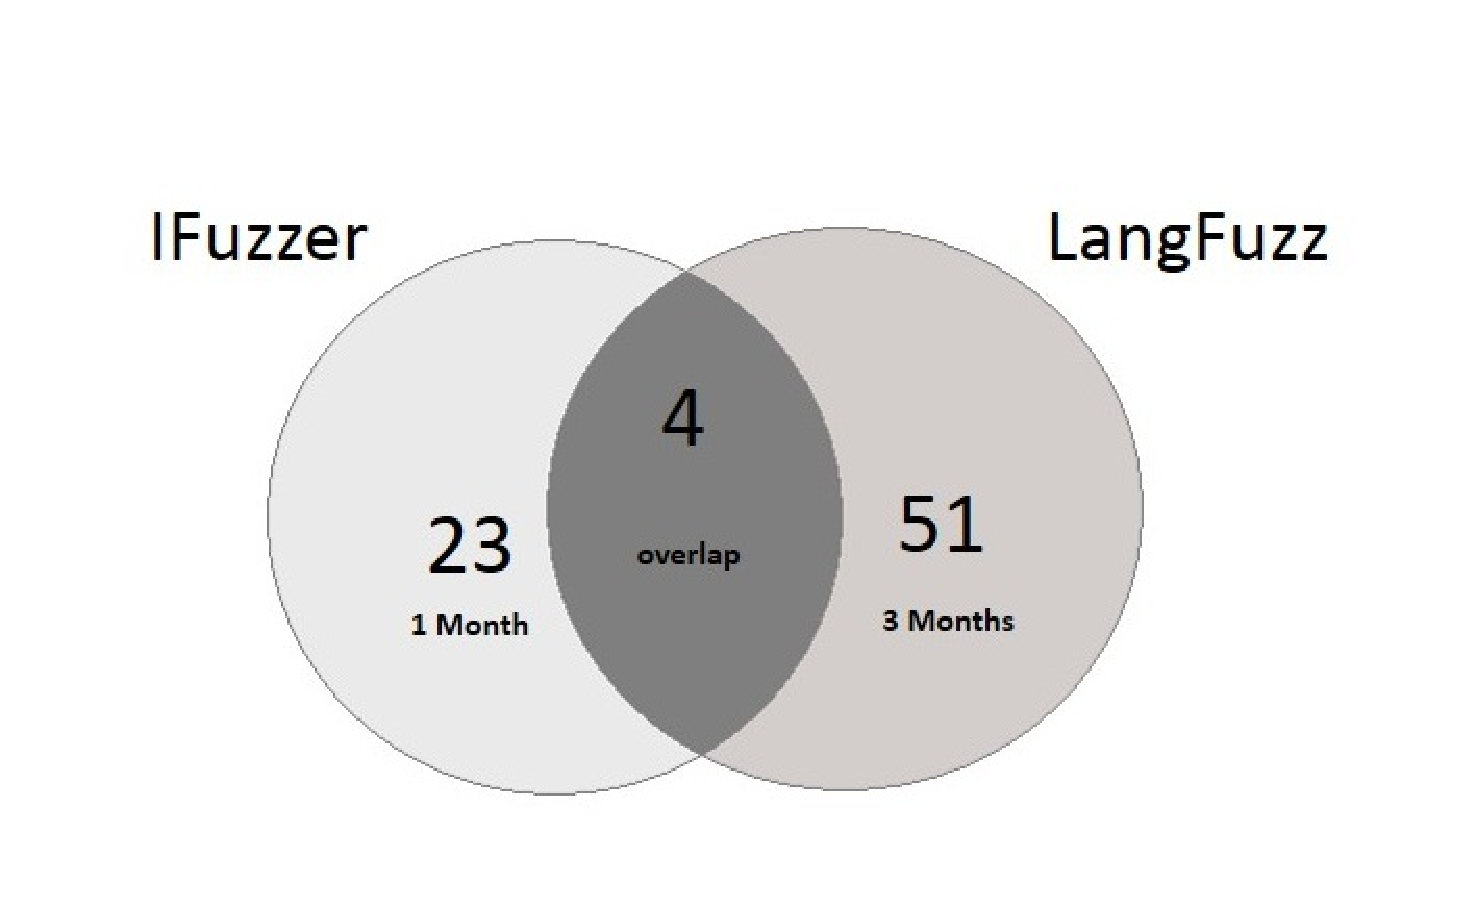
\epsfig{file=overlap.eps, height= 1.8in, width=3.5in}
\caption {Number of bugs found by both fuzzers and their overlap}
\label{fig5}
\end{figure}

\begin{figure}[h]
\centering
\rule{9cm}{0.5pt}
\epsfig{file=codesnippet2.eps, height= 0.80in, width=2.5in}
\rule{9cm}{0.5pt}
\caption {Test Case generated by IFuzzer crashing the Spidermonkey JavaScript engine. JavaScript engine fails to handle the situation, leading to memory leak }
\label{fig7}
\end{figure}

\indent The number of bugs found by IFuzzer shows the effectiveness of the evolutionary approach and it is as good as other generative approaches. 
IFuzzer tool shows that evolutionary approach which is similar to that of biological evolution is capable of generating programs with a given objective.\\
\indent With curiosity, when we ran on latest version of Spidermonkey IFuzzer found  4 bugs. One of the bug is accepted as severe bug (Bug Id: 1133247) \cite{Misc01} where one of the component fails to handle the situation and JavaScript engine consumes available heap memory and crashes in few seconds. Code fragment responsible for crash is shown in ~\autoref{fig7}

\section{Conclusion and Future Work} \label{conclusion}
In an approach to fuzz testing, IFuzzer uses an evolutionary code generation strategies that can be applied to any language provided with appropriate grammar specification and set of test cases for code generation process. The fuzzer uses objective function defined to help the fuzzer in reaching the goal in an efficient way. This makes the IFuzzer an effective tool. In our evaluation, it is shown that IFuzzer is fast in reaching objective and also it is as effective as other generative fuzzers. We recommend our approach for automated code generation for testing of any target language that can be expressed in grammar specification, this includes the software products like interpreters and compilers.\\
\indent We plan to investigate for more code parameters that can be considered for fitness evaluation. In our experiments we observed that genetic operations parameters must be tuned for further improvement in evolution process. This can be done on based of the observations and vary for different environments. Another improvement can be to keep track of more information on the program execution which helps to guide the fuzzer in better way. For example,  finding the tainted paths which gives coverage of functions executed, lines executed, paths that lead to a bug will be useful in code generation. Finally we intend to improve the code generation part and thereby extend its usage to more applications.

\subsubsection*{\textbf{Acknowledgments}} 
We thank many people who helped us to get this work done. First we would thank Christan Holler from Mozilla for his suggestions and comments. Furthermore thanks to anonymous reviewers who provided helpful feedback in writing this paper.

\bibliographystyle{abbrv}
\bibliography{sigproc}

\appendix
\section{Parameters} \label{AppendixA}
\begin{tabular}{ l c }
Parameter & Value \\
\hline

\end{tabular}

\end{document}